% this is chapter about the introduction about the problem in my thesis: it is
% the cardinality estimation to query performance.

\chapter{Query optimization}\label{chapter:query optimization}

\section{How is a query executed?}

\subsection{The main stages}

There are five main components in PostgreSQL architecture
\cite{pg_internals}:

\begin{description}
    \item[the parser]  parses the query string;
    \item[the rewriter] applies the rewrite rules (e.g.\ views);
    \item[the optimizer] determines an efficient query plan;
    \item[the executor] executes a query plan;
    \item[the utility processor] processes DDL such as {\bfseries CREATE TABLE}.
\end{description}

Figure 2.1 shows the architecture diagram of the query executor in PostgreSQL.
In the first stage, the query string is parsed into a parse tree by the parser.
After that, the query is then rewritten and checked semantically. In the next
stage, PostgreSQL processes DDL (Data Definition Language) like {\bfseries
CREATE TABLE} or applies rewrite rules in the rewriter. The query tree is used to
produce query plans and then the optimizer chooses the best plan based on a
specific criterion, such as estimated cost in cost-based optimizers. Finally, the
executor executes the plan chosen by the optimizer.

\begin{figure}[H]
    \centering
    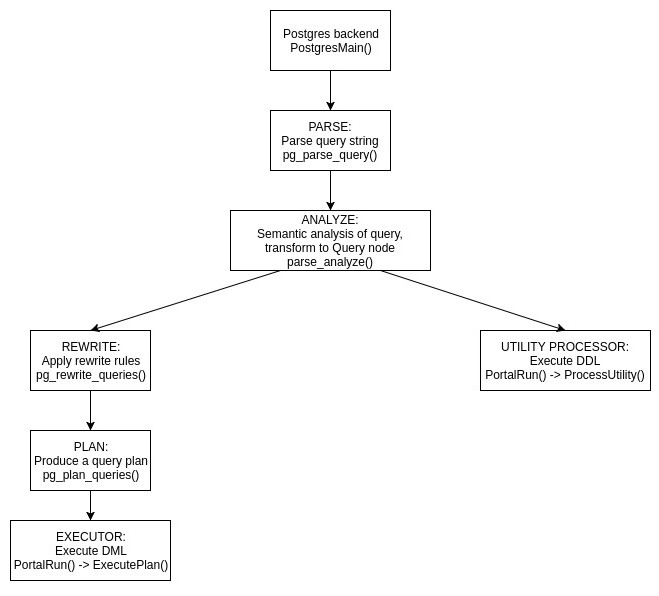
\includegraphics[width=1.0\textwidth]{architecture_diagram.jpg}
    \caption{Architecture diagram of PostgreSQL}
\end{figure}

\subsection{Parser}

The aim of the parser ~\cite{flow_of_a_select_statement} is to check the syntax of
the query string. If the syntax of the query string is valid, the parser build a parse
tree; whereas it returns an error. The syntax is defined in gram.y and scan.l which are built using the Unix tools yacc and lex. 

PostgreSQL uses Bison, the parsing technology used by Ruby. A parser code based on 
a series of grammar rules is generated by Bison during the PostgreSQL C build process.
The parser finds a corresponding pattern or syntax in the query string by checking each
grammar rule, and then inserts a new C memory structure into the parse tree data structure.

Figure 2.2 is an example of the below query's parse tree:
\begin{verbatim}
SELECT * FROM movies
WHERE country = 'France' ORDER BY id ASC LIMIT 1
\end{verbatim}

\begin{figure}[H]
    \centering
    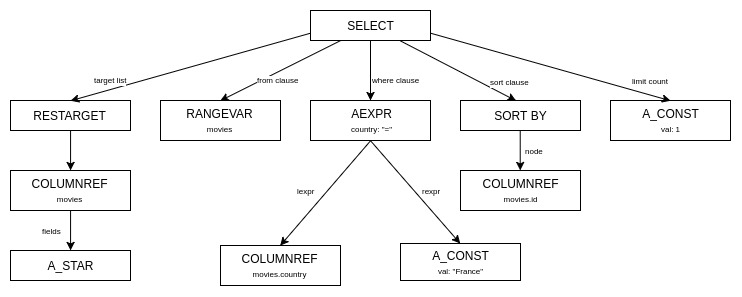
\includegraphics[width=1.0\textwidth]{parser_example.jpg}
    \caption{An example about parse tree.}
\end{figure}

\subsection{Rewriter}

After generating a parse tree, PostgreSQL converts this parse tree into another tree called as the query tree. A query tree contains parts ~\cite{pg_internals}:

\begin{itemize}
    \item The command type: it tells which command of the query string, such as
    	SELECT, INSERT, UPDATE, DELETE.
    \item The range table: it contains the relations that are used in the query.
    	For example, in a SELECT statement, the range table is the list of relations given after 
    	the FROM key word.
    \item The result relation: it is an index into the range table, which identifies
    	the relation where the results of the query go. In INSERT, UPDATE and DELETE statements,
    	the result relation is the relation where the changes are to take effect. There is not 
    	a result in SELECT queries.
    \item The target list: it contains expressions that define the result of the query. To
     	be more specific, in SELECT statement, the target list is a list of expression 	
     	between the key words SELECT and FROM. * is a special expression, it is just an 
     	abbreviation for all the column names of a relation.
    \item The qualification: it is an expression much like one of those contained in the target list 
    	entries. Its result value is a boolean, which tells whether the operation (INSERT, UPDATE, 
    	DELETE, or SELECT) for the final result row should be executed or not. In SQL statement, the qualification
    	is the WHERE clause.
    \item The join tree: it shows the structure of the FROM clause. 
    \item The others: the other parts of the query tree like the ORDER BY clause
\end{itemize}

Figure 2.3 is an example of the below query's query tree:
\begin{verbatim}
SELECT * FROM movies
WHERE country = 'France' ORDER BY id ASC LIMIT 1
\end{verbatim}

\begin{figure}[H]
    \centering
    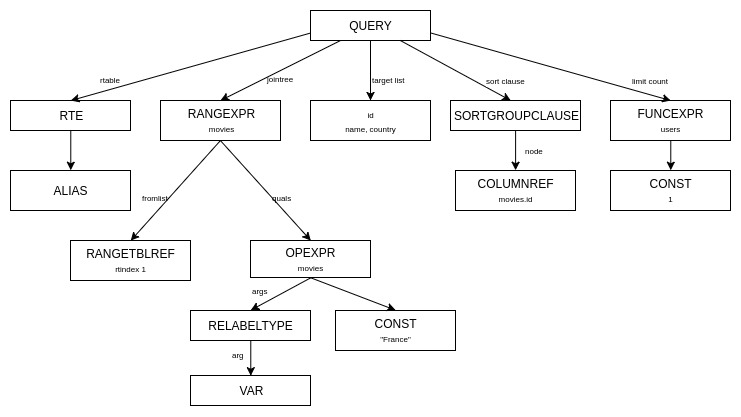
\includegraphics[width=1.0\textwidth]{example_querytree.jpg}
    \caption{An example about query tree.}
\end{figure}

\subsection{Planner/optimizer}

Planner's main task is to create an optimal execution plan. There are many 
ways which produce the same results to execute a query tree of a SQL plan. The query optimizer will
examine each these execution plans and finally choose the best execution plan based-on 
a specific criterion, such as estimated cost in cost-based optimizers (PostgreSQL's optimizer)
.In PostgreSQL, after the cheapest path is determined, a full-fledged plan tree is built to pass to the executor.

Figure 2.4 is the below query's full-fledged plan tree:
\begin{verbatim}
SELECT * FROM movies
WHERE country = 'France' ORDER BY id ASC LIMIT 1
\end{verbatim}

\begin{figure}[H]
    \centering
    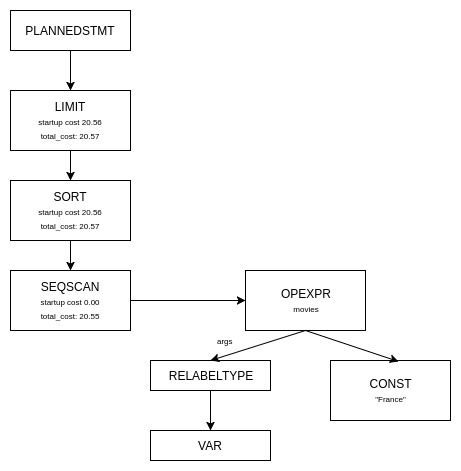
\includegraphics[width=0.7\textwidth]{plan_tree_example.jpg}
    \caption{An example about full-fledged plan tree.}
\end{figure}

\subsection{Executor}

The executor~\cite{pg_internals} takes the plan handed back by the planner and
recursively processes it to extract the required set of rows. This is
essentially a demand-pull pipeline mechanism. Each time a plan node is called,
it must deliver one more row, or report that it is done delivering rows.

When executing complex queries which involve many levels of plan nodes, each node computes and 
returns its next output row each time it is called. Each node is also responsible for applying 
any selection or projection expressions that were assigned to it by the planner.

\section{Query optimization}
\subsection{Introduction}

{\bfseries Query optimization} is a function of relational database management
systems. The query optimizer attempts to determine the most efficient way to
execute a given query by considering the possible query plans. Therefore, it is
belong to planner stage.

There are two factors that impact on the decision of the optimizer: the amount of time spent 
figuring out the best query plan and  the quality of the choice. Different qualities of database 
management systems have different ways of balancing these two. Cost-based query optimiers, such as 
PostgreSQL optimizer, evaluate the resource footprint of various query plans and use this as the 
basis for plan selection. They assign an estimated `cost' to each possible query plan, and choose 
the plan with the smallest cost. 

\subsection{The query optimizer of PostgreSQL}

As i mentioned above, PostgreSQL's optimizer is a cost-based optimizer, so it
chooses the plan that have the lowest estimated processing cost to execute.
PostgreSQL's optimizer determines the cost of executing a query plan based on
two main factors:

\begin{itemize}
    \item Cardinality estimation: the total number of rows processed at each
        level of a query plan, referred to as the cardinality of the plan.
    \item Cost model: the cost model of the algorithm dictated by the operators
        used in the query
\end{itemize}

The first factor, cardinality, is used as an input parameter of the second
factor, the cost model. Cardinality estimation has a bigger impact on query
performance than cost model~\cite{adaptive cardinality estimation}.

\subsection{PostgreSQL's cardinality estimator and its limitations}

\subsubsection{PostgreSQL's cardinality estimator}

Postgresql's optimizer follows the traditional textbook architecture. PostgreSQL's estimator
uses histograms (quantile statistic), most common values with their frequences and domain
cardinalities (distinct value counts) to estimate cardinalities of base tables. Histograms
can not be applied to estimate cardinalities of complex predicates. To combine conjenctive predicates
for the same table, independence assumption is used and PostgreSQL multiplies the selectivites of the
individual selectivity estimates.

There are some assumptions~\cite{JOB} in PostgreSQL's estimator:

\begin{description}
    \item[Independence:] predicates on attributes (in the same table or from
    joined tables) are independent.
    \item[Uniformity:] all values, except for the most-frequent ones, are assumed
    to have the same number of tuples
    \item[Principle of inclusion:] the domains of the join keys overlap such that
    the keys from the smaller domain have matches in the larger domain.
\end{description}

The formula~\cite{JOB} that is used to estimate result sizes of joins show these
assumptions:\\

\[
\vert T_{1} \bowtie_{x=y} T_{2}\vert =
\frac{{\vert {T_{1}\vert}}{\vert {T_{2}\vert}}}{\max(dom(x),dom(y))}
\]

Where $T_{1}$ and $T_{2}$ are arbitrary expresions and $dom(x)$ is the domain
cardinality of attribute $x$, i.e., the number of distinct values of $x$.

\subsubsection{The limitation of PostgreSQL's cardinality estimator}

\begin{itemize}
    \item Correlated data: Correlated data~\cite{CE limitations} between
        columns can lead to PostgreSQL estimator's bad cardinality estimates. To
        be more specific, I use the example below to show the impact of the
        correlation between relations on cardinality estimation of PostgreSQL\@:       
		\begin{verbatim}
        SELECT * FROM Products
        WHERE Company = 'Toyota' AND Brand = 'Civic'
        \end{verbatim}	           
        When you look at this query, you will know immediately how many rows are
        returned. The number of returned results is zero because the company
        Toyota doesn't have Civic brand. But as i mentioned above, PostgreSQL's
        optimizer assumes uniformity, independence, inclusion, so it looks at
        each search predicate indepedently.

        In the first step the estimator makes the cardinality selectivity for the predicate
        {\bfseries Company = `Toyota'}. After that, the estimator produces a
        cardinality selectivity for the predicate {\bfseries Brand = `Civic'}.
        Finally, the estimator computes the cardinality selectivity of the query by 	
        multiplying the cardinality selectivities . For example, if 0.4, 0.4 are 		
        respectively the cardinality selectivity of the first and second predicate, the 
        final cardinality selectivity will be 0.16 (0.4*0.4) instead of 0.0 as the fact. The 
        PostgreSQL's optimizer handles every predicate on its own without any correlation
        between relations.
\end{itemize}
